\subsection{Simulator}

In diesem Kapitel wird das Erarbeiten des Konzeptes des Simulators, der Implementierung und der Resultate festgehalten.


\subsubsection{Spezifikationen}

Die folgenden Spezifikationen soll der Simulator erfüllen.

\begin{table}[H]
\centering
\small
\begin{tabularx}{\textwidth}{|l|X|l|}
\hline
  \textbf{Nr.} & \textbf{Spezifikation} & \textbf{Priorität 1-3}  \\
  \hline
  1  & Der Zielknoten kann ausgewählt werden. &  2\\
  \hline
   2   & Der Roboter speichert den Graph intern.  & 1\\
  \hline
   3 & Der Roboter überprüft seine Nachbarsknoten.&1\\
  \hline
  4 & Der Roboter erkennt fehlende Linien und reagiert darauf. & 1\\
  \hline
  5 &   Der Roboter erkennt Pylonen und reagiert darauf. & 1\\
  \hline
   6  &   Der Roboter erkennt Barrieren und reagiert darauf. & 1\\
  \hline
    7 &   Der Roboter berechnet den kürzesten Weg im Graphen.& 1\\
  \hline
     8  &   Der Weg des Roboters wird im GUI angezeigt. & 1\\
  \hline
      9   &   Die Reaktionen auf die Hindernisse werden im GUI angezeigt. & 2\\
  \hline
 10   &   Die Hindernisse werden im GUI angezeigt. & 2\\
  \hline
   11   &   Die Reihenfolge der Knoten wird erkannt, als Vorbereitung, dass der Roboter, der Steuerung sagen kann, wo sich der nächste Weg befindet. & 3\\
  \hline

\end{tabularx}
\caption{Spezifikationen Simulator}
\label{table:spezifikation-simulator}
\end{table}

\subsubsection{Konzeption}

Mit einem morphologischen Kasten (siehe Anhang \ref{mk-simulator}) wurden mehrere Varianten ermittelt, die alle die Spezifikationen erfüllen können. Mit einer Nutzwertanalyse(siehe Anhang \ref{nutzwertanalyse}) wurde die beste Variante bestimmt.

\begin{itemize}
    \item Programmiersprache: Python
    \item Wegnetz einlesen: YAML
    \item Wegnetz intern speichern: Key-Values
    \item Bewegliche Hindernisse erfassen: Gewichtung
    \item Blockierte Knoten erfassen: Knoten entfernen
    \item Wegfindung: eigene Implementation
    \item Clientseitige Kommunikation \acrshort{i/o}: GUI
\end{itemize}

Die einzelnen Tätigkeiten wurden in GitHub Issues festgehalten. Die einzelnen Features wurden unter den Entwickelnden aufgeteilt und via GitHub Issues assigned. So ist sichtbar, wer woran arbeitet.

\begin{figure}[H]
\centering
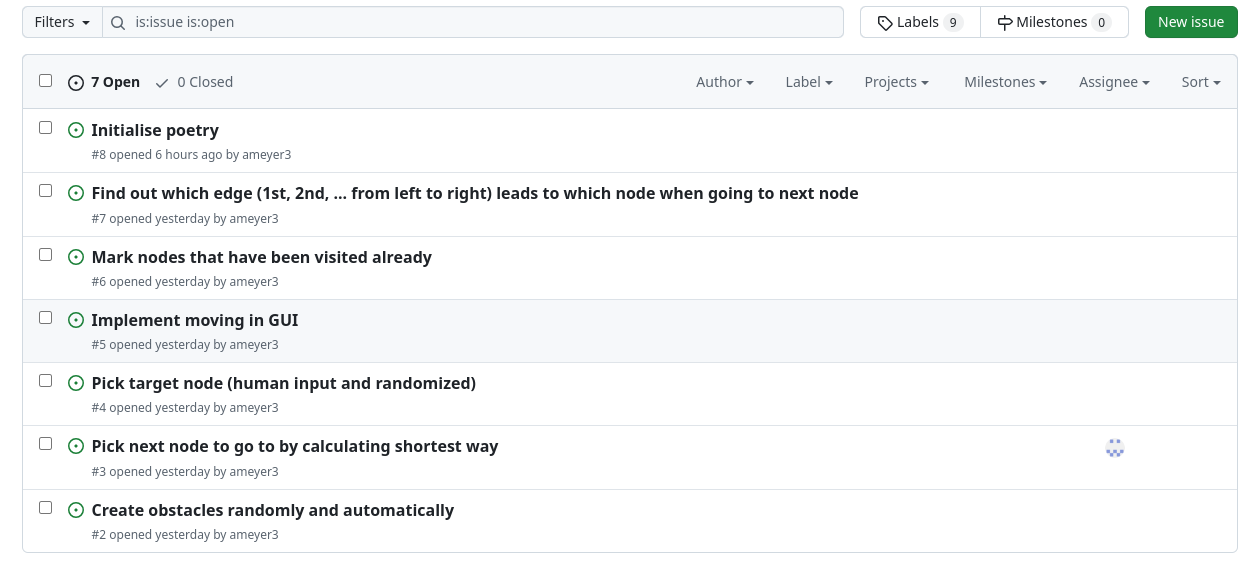
\includegraphics[width=\textwidth]{img/github-issues.png}
\caption{Ausschnitt GitHub Issue Liste}
\label{fig:github-issues}
\end{figure}

Es wurde ein objektorientierter Ansatz gewählt, um den Simulator umzusetzen. Die Roboter-klasse soll dabei den physischen Roboter darstellen, der die einzelnen Bauteile besitzt. So soll zum Beispiel die Wheels-Klasse als Simulation für das Drehen und Fortbewegen dienen. An diese Klasse werden die Nachrichten gesendet, welche im echten Roboter an die elektrische Steuerung des Motors gesendet werden würden.

Es gibt zusätzlich zum normalen Modus (\verb|run_normal_mode|) auch einen Modus, in dem der Roboter sich blind durch den Graphen bewegt, falls er nicht mehr weiss, wo er sich befindet (\verb|run_blind_testing_mode|). Dieser wird im folgenden Abschnitt ``Trial and Error'' noch weiter erklärt. Im Klassendiagramm sind die Methoden im Roboter so dargestellt, dass diese Methoden, die nur für einen bestimmten Modus verwendet werden, direkt unterhalb der oeffentlichen \verb|run| Methode ist. Diese Methoden, die sich zuunterst befinden, werden von allen Modi verwendet. 

TOOD explain the diagram moree

\begin{figure}[H]
\centering
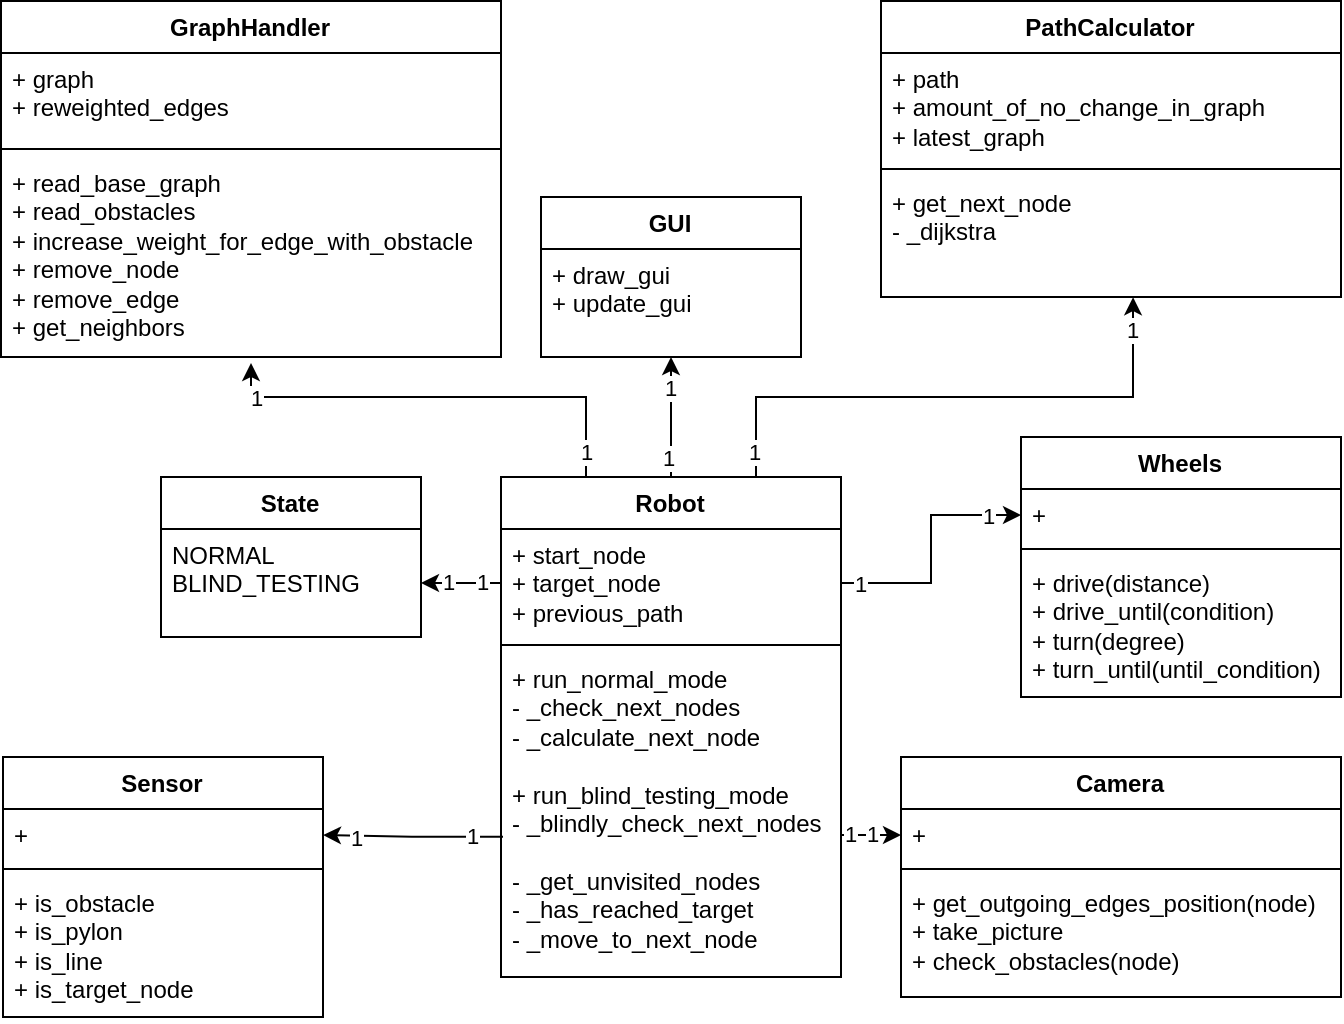
\includegraphics[width=\textwidth]{assets/informatik-prototyp/simulator/simulator-erd.png}
\caption{Simulator Klassendiagramm}
\label{fig:simulator-classdia}
\end{figure}

\subsubsection{Entwicklung}

Der erste Schritt ist es einen Graph zu definieren. Dazu wird ein YAML File mit dem konfigurierten Graph erstellt. 
Dazu wird der vorgegebene Graph beschriftet: Jeder Knoten erhält einen Buchstaben und jede Kante ein Gewicht. Die Gewichtungen sind die Längen der Strecken in Millimeter. Diese Beschriftung wird wie folgt in einem YAML File beschrieben.

\begin{figure}[H]
\begin{subfigure}{0.35\textwidth}
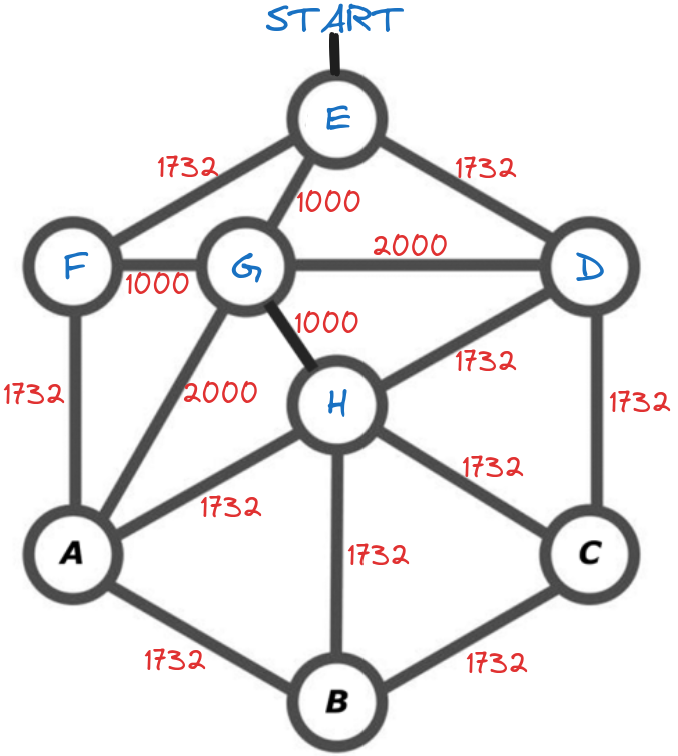
\includegraphics[width=0.95\linewidth]{img/graph_with_weighted_edges_1.png} 
\caption{Beschrifteter Graph}
\label{fig:labeled-graph}
\end{subfigure}
\begin{subfigure}{0.720\textwidth}
\begin{footnotesize}
\begin{verbatim}
START: { E: 300 }
A: { F: 1732, G: 2000, H: 1732, B: 1732 }
B: { A: 1732, H: 1732, C: 1732 }
C: { D: 1732, B: 1732, H: 1732 }
D: { E: 1732, C: 1732, H: 1732, G: 2000 }
E: { START: 300, D: 1732, G: 1000, F: 1732 }
F: { E: 1732, G: 1000, A: 1732 }
G: { E: 1000, D: 2000, H: 1000, A: 2000, F: 1000 }
H: { G: 1000, D: 1732, C: 1732, B: 1732, A: 1732 }
\end{verbatim}
\end{footnotesize}
\caption{Graph in YAML}
\label{fig:graph-yaml}
\end{subfigure}
\end{figure}

Die Hindernisse und die fehlenden Linien sind ebenfalls in einem YAML File definiert. So können diese einfach angepasst werden:

\begin{verbatim}
cone:
  - F
barrier:
  - [E, G]
missing_line:
  - [E, D]
\end{verbatim}

Der Simulator liest die beiden Dateien ein und speichert sie intern als Python Dictionaries.

\textbf{Ablauf des Simulators}

Das Ziel ist es, dass der Ablauf möglichst nah an dem Ablauf des Gesamtkonzeptes herankommt.
Der Programmablauf besteht aus folgenden Teilen:
\begin{enumerate}
    \item Nachbarsknoten auf Hindernisse prüfen
    \item Nächste Knoten berechnen
    \item Zu nächstem Knoten fahren
\end{enumerate}

Es wird simuliert, dass der Roboter auf einem Knoten steht. Er dreht sich im Uhrzeigersinn im Kreis und prüft alle Nachbarsknoten. In der Simulation wird dafür das Hindernis-Dictionary auf die jeweiligen Knoten und Strecken geprüft. Falls ein Hindernis detektiert wird, reagiert er wie folgt:

\begin{itemize}
    \item Ein Pylon steht auf dem Nachbarsknoten: Dieser Knoten und alle Kanten, die dahin führen, werden im intern gespeicherten Graph-Dictionary entfernt.
    \item Eine Barriere wird auf einer ausgehenden Strecke erkannt: Die Strecke wird im intern gespeicherten Graph-Dictionary höher gewichtet. Die Höhe der neuen Gewichtung widerspiegelt sich im Verhältnis zur Zeit die das zusätzliche Abhandeln des Objektes entspricht.
    \item Eine ausgehende Linie fehlt: Diese Verbindung wird aus dem intern gespeicherten Graph entfernt.
\end{itemize}

Falls noch nie eine Berechnung des kürzesten Weges durchgeführt wurde oder sich der intern gespeicherte Graph verändert hat, wird die Berechnung des kürzesten Pfades mittels Dijkstra durchgeführt. Der geplante Pfad sowie der nächste Knoten werden dabei gespeichert.

Danach bewegt sich der Roboter zum nächsten Knoten. Dabei wird simuliert, dass sich der Roboter zur nächsten Linie drehen soll und die Distanz zum nächsten Knoten fahren soll. Im Simulator sind alle Kanten eines Knotens im Uhrzeigersinn angeordnet gespeichert. Die Position (relativ zu der Strecke, von der der Roboter herkommt) der nächsten Strecke wird mit dem Ring Buffer \footnote{\url{https://en.wikipedia.org/wiki/Circular\_buffer}} zirkulär berechnet. So kann simuliert werden, dass eine Liste in einem Kreis angeordnet ist. So wird es in der richtigen Applikation möglich sein, die Kanten zu identifizieren. 

\begin{figure}[H]
\centering
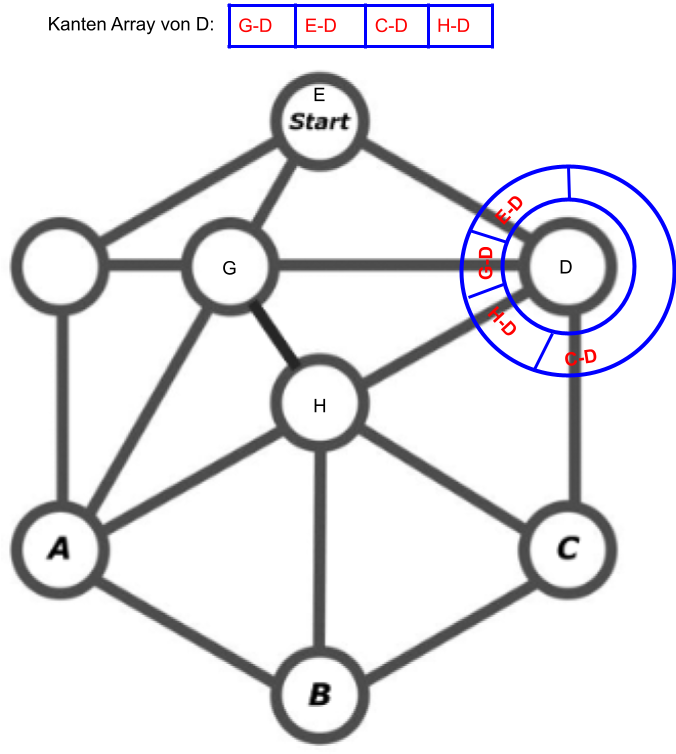
\includegraphics[width=0.5\textwidth]{assets/informatik-prototyp/simulator/ring-buffer-graph.png}
\caption{Graph with Ring Buffer}
\label{fig:ring-buffer-graph}
\end{figure}

Die Position relativ zu einer bestimmten Kante herauszufinden wird wie folgt implementiert:

\begin{verbatim}
edges_to_target = (target_index - start_index) % len(neighbors)
\end{verbatim}

Dieser Ablauf wird so lange wiederholt, bis der Zielknoten erreicht wird.
Während des ganzen Ablaufes werden die einzelnen Klassen aufgerufen, welche die die einzelnen Roboterbauteile simulieren. In diesen befindet sich zum Teil eine Mock-Logik (zum Beispiel Hindernisse aus dem Konfigurationsfile lesen anstatt aus Bildern von der Kamera detektieren) und oft nur simple Print-Statements. Diese Print-Statements sollen die Schnittstelle zu der Elektronik simulieren.

\textbf{Trial and Error Mode}

Ein Modus BLIND\_TESTING wurde implementiert, der aktiviert wird, wenn der Roboter nicht mehr weiss, wo er sich befindet. Dieser Modus dient im realen Roboter als Risikominderung. Dabei wird der Roboter die Hindernisse und Knoten gleich erkennen, wie im normalen Modus, jedoch wird nicht der schnellste Weg berechnet. Der Roboter kennt alle ausgehenden Kanten des nächsten Knotens und die Hindernisse, die sich darauf befinden. Er wird nun jeweils ohne Berechnung die erste Kante, die nicht zu einem Pylonen führt, von links aus nehmen und so blind den Graphen traversieren, bis mit der Kamera der richtige Zielknoten erkannt wird.

\textbf{Technische Aspekte}\label{technical-aspect-simulator}

Um die Abhängigkeiten zu externen Bibliotheken zu organisieren wird Poetry\footnote{\url{https://python-poetry.org/}} verwendet. Dabei werden die Bibliotheken in eine virtuelle Umgebung installiert, worin der Simulator ausgeführt wird.

\textbf{Graphical User Interface}

Das GUI wurde mit PyGame\footnote{\url{https://www.pygame.org/news}} umgesetzt. Der Graph wird mit beschrifteten Knoten dargestellt. Der Roboter wird als ein Kreis mit einem Dreieck dargestellt. Die Spitze des Dreiecks zeigt die Richtung, in welche der Roboter schaut.
Die Fahrt des Roboters auf den Linien ist ebenfalls dargestellt.

Auf folgendem Bild dreht sich unser Roboter auf der Stelle im Kreis, um die umliegenden Knoten und Kanten zu überprüfen.
Das orange Dreieck stellt eine Pylone dar, das rote Rechteck ein Hindernis, das beseitigt werden kann und das rote Kreuz ist eine Linie, die fehlt. Die rote Fahne ist das Ziel, das der Roboter erreichen soll.

\begin{figure}[H]
\begin{subfigure}{0.49\textwidth}
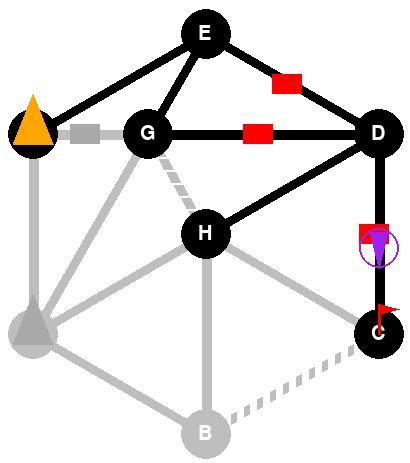
\includegraphics[width=0.95\textwidth]{assets/informatik-prototyp/simulator/sim-ui.png}
\caption{GUI des Simulators}
\label{fig:sim-gui}
\end{subfigure}
\begin{subfigure}{0.49\textwidth}
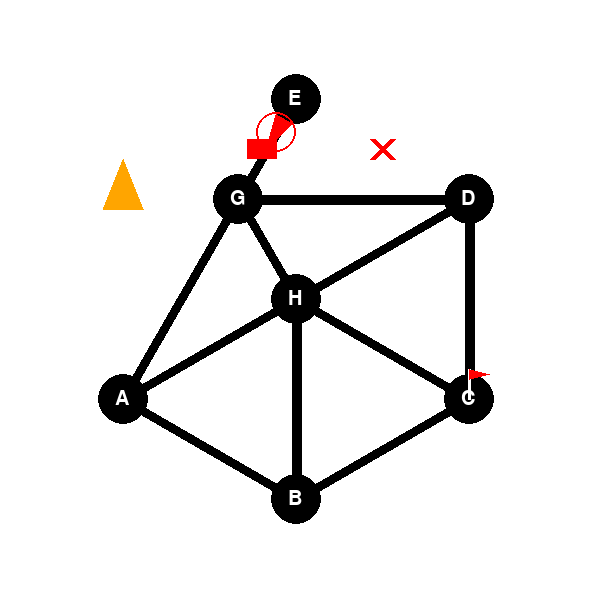
\includegraphics[width=0.95\textwidth]{assets/informatik-prototyp/simulator/removed-lines-sim.png}
\caption{GUI des Simulators unbefahrbare Linien entfernt}
\label{fig:sim-gui-removed-lines}
\end{subfigure}
\end{figure}

\subsubsection{Simulation}

In diesem Abschnitt wird erläutert wie der Simulator aufgesetzt wird, und wie man diesen verwendet. Zusätzlich haben wir automatisierte Testdurchläuffe durchgeführt, welche Ergebnisse anschliessend Dokumentiert sind.

\textbf{Voraussetzungen und Installation}

Wie in Kapitel \ref{technical-aspect-simulator} erwähnt, wird unser Simulator in einer Virtuellen Python Umgebung ausgeführt. Um diese Virtuelle Python Umgebung zu nutzen müssen vorerst nachfolgende Software installiert sein:

\begin{itemize}
    \item Python Version 3.9 oder neuer
    
    \url{https://www.python.org/}
    \item Poetry Version 1.8 oder neuer
    
    \url{https://python-poetry.org/}
\end{itemize}

Sofern dies installiert ist, kann im Grundverzeichnis des Simulators der nachfolgende Befehl ausgeführt werden, um die Abhängigkeiten zu installieren

\begin{verbatim}
poetry install
\end{verbatim}

\textbf{Simulator ausführen}

Sind die Vorbedingungen erfüllt, kann im Grundverzeichnis Simulators nachfolgender Befehl ausgeführt werden, um eine einfache Simulation zu starten:

\begin{verbatim}
poetry run python -m simulator
\end{verbatim}

Um die Hilfe anzuzeigen kann das Argument \verb|--help| angegeben werden. Somit werden alle Optionen welche der Simulator bietet angezeigt.:


\begin{footnotesize}
\begin{verbatim}
poetry run python -m simulator --help
usage: simulator [-h] [-s START_NODE] [-t {A,B,C}] [-r] [-c CONES] [-b BARRIERS] 
[-l MISSING_LINES] [--no-gui] [--speed SPEED] [--time-multiplier TIME_MULTIPLIER] 
[--simulate-time] [--verbose]

PREN1 Simulator

options:
  -h, --help                        show this help message and exit
  -s START_NODE, --start-node START_NODE
  -t {A,B,C}, --target-node {A,B,C}
  -r, --random                      Generate random obstacles
  -c, --cones CONES                 if random: Number of cones to add
  -b, --barriers BARRIERS           if random: Number of barriers to add
  -l, --missing-lines MISSING_LINES if random: Number of missing-lines to add
  --no-gui                          Run simulation without gui
  --speed SPEED                     Speed of the robot in mm/s
  --time-multiplier TIME_MULTIPLIER multiplier for all simulations
  --simulate-time                   Simulate time for task that the robot does
  --verbose                         Prints the single steps
\end{verbatim}
\end{footnotesize}

Dies gibt uns Hinweise über alle Möglichen Aktionen. Die wichtigsten nachfolgend erklährt:

\begin{itemize}
    \item \verb|--random| ermöglicht das automatisch generieren von Hindernissen.
    \item \verb|--cones|, \verb|--barriers|, \verb|--missing-lines| bestimmt, wie viele Hindernisse im generierten Graph platziert werden. Standardmässig werden jeweils 2 Stück platziert.
    \item \verb|--no-gui| und \verb|--simulate-time| wird verwendet um den Simulator ohne grafisches User Interface durchlaufen zu lassen. Die Simulation wird in dem Verfahren so schnell wie möglich ausgeführt. Dies ist äussert hilfreich wenn hunderte, oder tausende Simulationen durchgeführt werden sollen.
    \item \verb|--verbose| ermöglicht Debugging-Ausgaben des Simulators in der Konsole.
\end{itemize}

Jede Ausführung gibt jeweils auch Informationen über den Verlauf der Simulation. Nachfolgend ein Ausschnitt einer Ausgabe:

\begin{footnotesize}
\begin{verbatim}
...
......
.........
[2024-12-26 16:47:56,305] DRIVE 816.0MM.
[2024-12-26 16:48:00,409] DRIVE -100MM.
[2024-12-26 16:48:01,932] DRIVE 100MM.
[2024-12-26 16:48:02,451] [ET] I am now infront of my next node B. I will now check for 
    the next 1 connections.
[2024-12-26 16:48:02,451] TURN -60 DEGREES.
[2024-12-26 16:48:04,134] TAKE PIC
[2024-12-26 16:48:04,134] Planned path is ['A', 'B', 'C']
[2024-12-26 16:48:04,134] The next node considering the shortest path is node C
[2024-12-26 16:48:04,134] Moving from B to C which is 0 degrees from current direction
[2024-12-26 16:48:04,134] TURN 0 DEGREES.
[2024-12-26 16:48:04,136] DRIVE 1732MM.
[2024-12-26 16:48:12,820] DRIVE -100MM.
[2024-12-26 16:48:14,353] Expected a line from node C to D with angle 0deg
[2024-12-26 16:48:14,353] DRIVE 100MM.
Reached the target C via ['START', 'E', 'D', 'E', 'F', 'A', 'B', 'C']
traversing the graph took 84.728 seconds
\end{verbatim}
\end{footnotesize}

Bei erfolgreichem traversieren des Graphen wird am Ende den gesamten Pfad sowie die benötigte Zeit dafür ausgegeben.

Der Verlauf kann auch im Grafischen User Interface verfolgt werden. Dabei sind in Farbe die Hindernisse welche bereits erkennt worden sind. Sowie schwarz der Pfad der bekannt ist. Grau hingegen sind alle Pfade und Hindernisse welche zu dem Zeitpunkt noch unbekannt sind.
Die Anzeige aktualisiert sich in Echtzeit.
\begin{figure}[H]
    \centering
    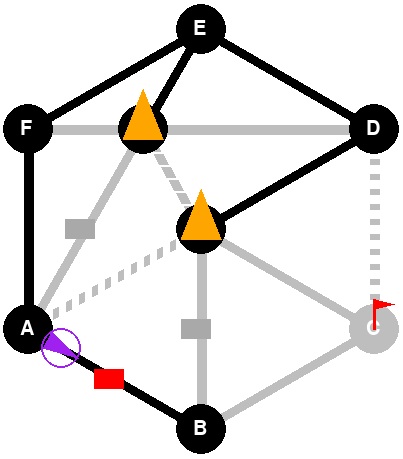
\includegraphics[width=0.5\linewidth]{assets//informatik-prototyp//simulator/simulator-run.png}
    \caption{GUI während Simulation}
    \label{fig:simulation-run}
\end{figure}

\textbf{Benchmark}

Durch das setzen des \verb|--random| Arguments können wir nun also auch zufällig generierte Graphen erstellen und diese traversieren.
Wenn wir auch noch \verb|--simulate-time| mitgeben, wird die Ausführungszeit zusätzlich simuliert.
Somit können wir fast unbegrenzt mögliche Graphen erstellen und die traversierung mit unserem Roboter in der selben Sekunde simulieren.

Dies haben wir nun mit nachfolgenden Optionen durchgeführt:

\begin{itemize}
  \item Anzahl Pylonen: 0-6
  \item Anzahl Barrieren: 0-14
  \item Anzahl fehlende Kanten: 0-13
  \item Zielknoten: A, B oder C
\end{itemize}

Mit allen möglichen Optionen wurden so 100'000 Durchläufe simuliert.
Für uns ist dabei wichtig, dass wir unter einer Laufzeit von 4 Minuten stehen, egal welcher Graph mit welchen Hindernissen wir Traversieren müssen.

Nachfolgend dazu die Auswertung dieser Durchläufe:

\begin{figure}[H]
  \centering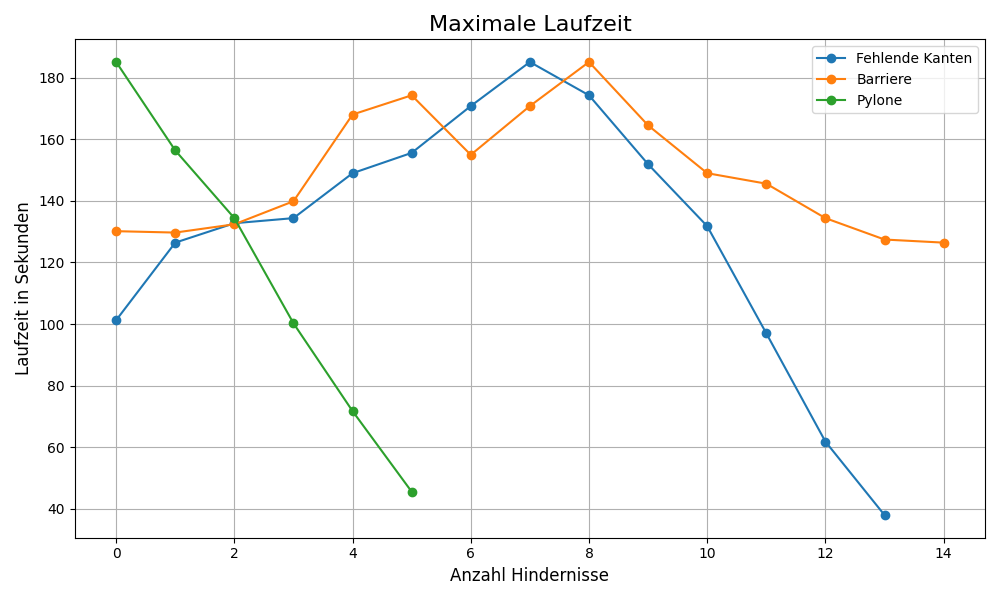
\includegraphics[width=0.75\linewidth]{assets/informatik-prototyp/simulator/max_seconds.png}
  \caption{Maximale benötigte Zeit}
  \label{fig:simulation-run-max-seconds}
\end{figure}

\begin{figure}[H]
  \centering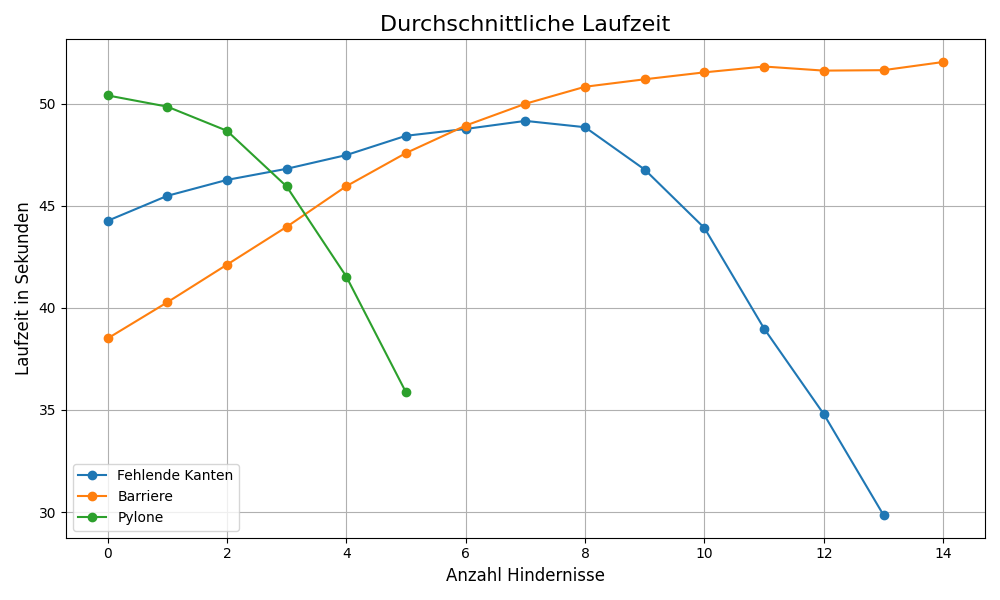
\includegraphics[width=0.75\linewidth]{assets/informatik-prototyp/simulator/mean_seconds.png}
  \caption{Durchschnittlich benötigte Zeit}
  \label{fig:simulation-run-mean-seconds}
\end{figure}

Wie zu sehen ist, brauchen wir im worst case ungefähr 185 Sekunden für das Traversieren. 
Die Durchschnittszeit ist jedoch viel besser und konstant unter 60 Sekunden.
Somit können wir davon ausgehen, dass unser Roboter mit der aktuellen Strategie den Graphen problemlos in der geforderten Zeit erfolgreich traversieren kann.

TODO HOW YO RUN SIMULATOR WITH ALL THE PARAMS

TODO document simulation runs + Ergebnisse (ev in Tabelle ''Testprotokoll'')